\documentclass[11pt,a4paper]{article}
\usepackage[utf8]{inputenc}
\usepackage[T1]{fontenc}
\usepackage[provide=*,ngerman]{babel}
\usepackage{lmodern,microtype,amsmath,amssymb,booktabs,tabularx,array,xcolor,fancyhdr,geometry,graphicx,hyperref}
\geometry{left=20mm,right=20mm,top=20mm,bottom=21mm}
\definecolor{ink}{HTML}{173643}\definecolor{teal}{HTML}{08786F}\definecolor{muted}{HTML}{53636B}\definecolor{pale}{HTML}{EFF6F5}
\hypersetup{colorlinks=true,urlcolor=teal,linkcolor=teal,pdftitle={CST Staubball: Klassik und Rueckwirkung v0.1},pdfauthor={X6 Astrolabium Arbeitsdokument}}
\pagestyle{fancy}\fancyhf{}\fancyfoot[L]{\small\sffamily\color{muted}X6 Astrolabium · Klassik und Rückwirkung v0.1}\fancyfoot[R]{\small\thepage/6}
\renewcommand{\headrulewidth}{0pt}
\setlength{\parindent}{0pt}\setlength{\parskip}{5pt}\setlength{\emergencystretch}{2em}
\newcolumntype{Y}{>{\raggedright\arraybackslash}X}
\newcommand{\kicker}[1]{{\sffamily\small\bfseries\color{teal}#1}\par}
\newcommand{\tit}[1]{{\sffamily\LARGE\bfseries\color{ink}#1}\par\vspace{6pt}}
\newcommand{\sect}[1]{\par\vspace{6pt}{\sffamily\large\bfseries\color{ink}#1}\par}
\newcommand{\note}[1]{\par\vspace{4pt}\colorbox{pale}{\parbox{\dimexpr\linewidth-2\fboxsep}{#1}}\par}
\begin{document}
\kicker{FORSCHUNGSPRÜFUNG · 5. NOVEMBER 2026}
\tit{Entstehen klassische Staubbewegung\\und gravitative Rückwirkung?}
\textbf{Befund: in der reduzierten Referenz ja; aus der vollständigen Kausalset-Summe bislang nicht nachgewiesen.}
Die mit der Historiengewichtung eingeführte Einstein-Staub-Referenz besitzt den richtigen klassischen Kollaps und die richtige Abhängigkeit von der Staubmasse. Der normierte Quantenkern reproduziert diese Bewegung in den hier geprüften semiklassischen Zuständen vor der Singularität. Die Referenz wurde aus einer bereits gravitativen Wirkung abgeleitet; sie ist noch kein Emergenznachweis aus diskreten Kausalsets.

\sect{Entscheidung nach der ausgeführten Prüfung}
\begin{tabularx}{\linewidth}{@{}>{\raggedright\arraybackslash}p{48mm}Y@{}}\toprule
\textbf{Frage} & \textbf{Ergebnis}\\\midrule
Klassische Staubbewegung & \textbf{PASS, bedingt.} Variation der gekoppelten Wirkung liefert Geodäten, Massenerhaltung und im homogenen Sektor die Friedmann-Gleichungen.\\
Grenzfall des reduzierten Kerns & \textbf{PASS im Referenztest.} 90 Zustandsauswertungen, drei zentrale Massen, drei Werte von $\hbar$, zwei Gitter; Vergleich mit unabhängiger analytischer Lösung.\\
Materie als Gravitationsquelle & \textbf{PASS in derselben Referenz.} Die Anfangszwangsgleichung und die Beschleunigung hängen von $M$ ab. Vierfache Masse verdoppelt $|\dot{\sqrt V}|$ bei gleichem Anfangsvolumen.\\
Klassik aus der 4D-CST-Summe & \textbf{HOLD.} Vollständiger Materie-Geometrie-Kern, physikalische Vergröberung und kontrollierter Grenzübergang fehlen.\\
Rückwirkung im endlichen CST-Modell & \textbf{HOLD.} Massenabhängige Endamplituden sind reproduzierbar, beweisen jedoch noch keine Einstein-Staub-Dynamik.\\\bottomrule
\end{tabularx}

\sect{Ein neuer Befund am bisherigen Historienträger}
Die festen frühen Werte $a(0)=1$, $a(0{,}4)=0{,}8$ bestimmen in der flachen klassischen Referenz den Kollapszeitpunkt $T_*=1{,}4061817646$. Der alte Katalog enthält ausschließlich positive Volumina bis $T=1{,}6$. Das gesamte alte Zeitfenster eignet sich deshalb nicht für einen Vergleich mit einer überall regulären klassischen Kollapslösung. Ein neuer Klassiktest muss zunächst \emph{vor} $T_*$ liegen.

\note{\textbf{Keine neue Bounce-Aussage.} Die reduzierte klassische Lösung erreicht weiterhin $V=0$ in endlicher Staubzeit. Die alte Ablehnung des dominanten Bounce-Kandidaten bleibt bestehen. Weder eine Randreflexion des Quantenkerns noch eine Massenantwort einzelner Zweige belegt Singularitätsauflösung.}

\newpage
\kicker{01 · VARIATION DES GEKOPPELTEN SYSTEMS}
\tit{Staub bewegt sich und erzeugt Krümmung}
Mit Signatur $(-+++)$, $c=1$, $\Lambda=0$ und irrotationalem Staub lautet die gewählte Kontinuumsreferenz
\[
 S=\frac{1}{16\pi G}\int d^4x\sqrt{-g}\,R+S_\partial
 -\frac12\int d^4x\sqrt{-g}\,\rho\left(g^{ab}\partial_aT\partial_bT+1\right).
\]
$S_\partial$ macht die festgelegte metrische Randvariation wohldefiniert. Die Rolle dynamischen Staubs als Zeit und Materie ist durch Brown und Kuchař [1] motiviert; hier wird ausdrücklich nur der irrotationale, später homogene Sektor verwendet.

\sect{Die vier Gleichungen entstehen gemeinsam}
Variation nach $\rho$, $T$ und $g^{ab}$, jeweils \emph{vor} Einsetzen der Normierungsbedingung, ergibt mit $u_a=-\partial_aT$
\[
 u^a u_a=-1,\qquad \nabla_a(\rho u^a)=0,\qquad
 G_{ab}=8\pi G\rho u_a u_b.
\]
Weil $\nabla_a u_b=\nabla_b u_a$, folgt zusätzlich
\[
 u^b\nabla_bu_a=u^b\nabla_a u_b=\tfrac12\nabla_a(u^b u_b)=0.
\]
Das sind druckloser geodätischer Transport, Massenerhaltung und gravitative Quellwirkung. Sie gelten für glatte Staubflüsse vor Kaustiken beziehungsweise Singularitäten. Ein auf einer schon vorgegebenen Geometrie transportierter Teststaub erfüllt allein noch nicht die letzte Gleichung.

\sect{Homogene Reduktion mit Zwangsgleichung}
Für eine flache periodische Zelle, $V=V_0a^3=q^2$ und $\kappa=3\pi G/2$, ist
\[
 L=-\frac{\dot q^2}{4\kappa N}
   +\frac{q^2\rho}{2}\left(\frac{\dot T^2}{N}-N\right),\qquad
 C=p_T-\kappa p_q^2=0.
\]
Im positiv orientierten Staubzweig gilt $p_T=M>0$. Erst nach Variation wählen wir $T=t$, $N=1$. Dann
\[
 H_{\rm phys}=-\kappa p_q^2,\qquad \dot q=-2\kappa p_q,
 \quad \dot p_q=0,\quad M=\kappa p_q^2=\text{konstant}.
\]
Für den Kollapszweig $p_q>0$ folgt
\[
 \boxed{q(T)=q_i-2\sqrt{\kappa M}(T-T_i)},\qquad \rho=\frac{M}{V}.
\]
Damit erhält man $H_a^2=8\pi G\rho/3$, $\ddot a/a=-4\pi G\rho/3$ und $\dot\rho+3H_a\rho=0$. Die freie Bewegung von $q$ bedeutet somit nicht fehlende Gravitation: Die nichtlineare Volumenkoordinate und der Zwang tragen deren Wirkung. Die periodische Zelle enthält weder Staubballoberfläche noch Außenraum.

\newpage
\kicker{02 · KLASSISCHER GRENZFALL DES GEWICHTETEN KERNS}
\tit{Die stationäre Phase liefert den Kollaps}
Für das bereits festgelegte Maß $dq=dV/(2\sqrt V)$ und den reduzierten Kern aus [3] lautet die diskretisierte Wirkung bei beliebigen positiven Zeitschritten
\[
 S_m=-\frac1{4\kappa}\sum_{j=0}^{m-1}
 \frac{(q_{j+1}-q_j)^2}{T_{j+1}-T_j}.
\]
Ihre innere Variation ergibt
\[
 \frac{\partial S_m}{\partial q_j}=\frac1{2\kappa}
 \left(\frac{q_{j+1}-q_j}{\Delta T_j}
       -\frac{q_j-q_{j-1}}{\Delta T_{j-1}}\right)=0.
\]
Der direkte stationäre Pfad ist also linear in $q$. Die Anfangsimpulspräparation wählt die Steigung; der Staubzwang ordnet ihr $M$ zu. Das Integrationsmaß allein bestimmt weder diese Masse noch die Einstein-Wirkung. Auf $q>0$ besitzt der gewählte Dirichlet-Kern zusätzlich Bildbeiträge; sie werden in der folgenden Prüfung durch eine weit vom Rand bleibende Präparation kontrolliert.

\sect{Festgelegter normierter Zustand}
Wir benutzen auf der Halbgeraden die normierte ungerade Bildkombination einer Gaußpackung mit $q_i=4$, $p_i=\sqrt M$, $\sigma_q^2=\hbar/2$ und $\kappa=1$. Die Zahlen sind dimensionslose Referenzeinheiten, keine neuen physikalischen Planckskalen. Die zentralen klassischen Massen sind $M=1/4,1,4$; $\hbar=0{,}04,0{,}02,0{,}01$. Für die volle Gerade gilt exakt
\[
 q_c=4-2p_iT,\qquad
 \sigma_q^2(T)=\frac\hbar2+2\hbar T^2,\qquad
 \langle V\rangle=q_c^2+\sigma_q^2(T).
\]
Die Halbgeradenlösung wird unabhängig durch die exakte Bildformel berechnet. Im geprüften Fenster $0\le T\le1/2$ bleibt der Schwerpunkt mindestens zehn Standardabweichungen von $q=0$ entfernt. Bildkorrekturen sind damit für die ausgewiesenen numerischen Fehler unerheblich. Für festes Zeitfenster vor $q_c=0$ verschwinden Breite und Volumenkorrektur mit $\hbar\to0$; dies ist eine kontrollierte semiklassische Familie des \emph{reduzierten} Modells.

\sect{Masse und Präparation müssen zusammenpassen}
Eine lokalisierte Packung ist kein scharfer Masseneigenzustand: Bis auf exponentiell kleine Bildkorrekturen ist $\langle\widehat M\rangle=M+\hbar/2$, wobei $\widehat M=-\widehat H$. Diese Energieerwartung wurde spektral geprüft. Der Vergleich gilt zur zentralen klassischen Masse $M$; die zusätzliche Streuung verschwindet im Grenzfall. Wer bei festem $q_i$ die Masse verändert, muss den Anfangsimpuls ändern. $M$, $q_i$ und $\dot q_i$ können bei festem $G$ nicht unabhängig vorgegeben werden.

\newpage
\kicker{03 · AUSGEFÜHRTE REFERENZPRÜFUNGEN}
\tit{Unabhängige Rechnungen stimmen überein}
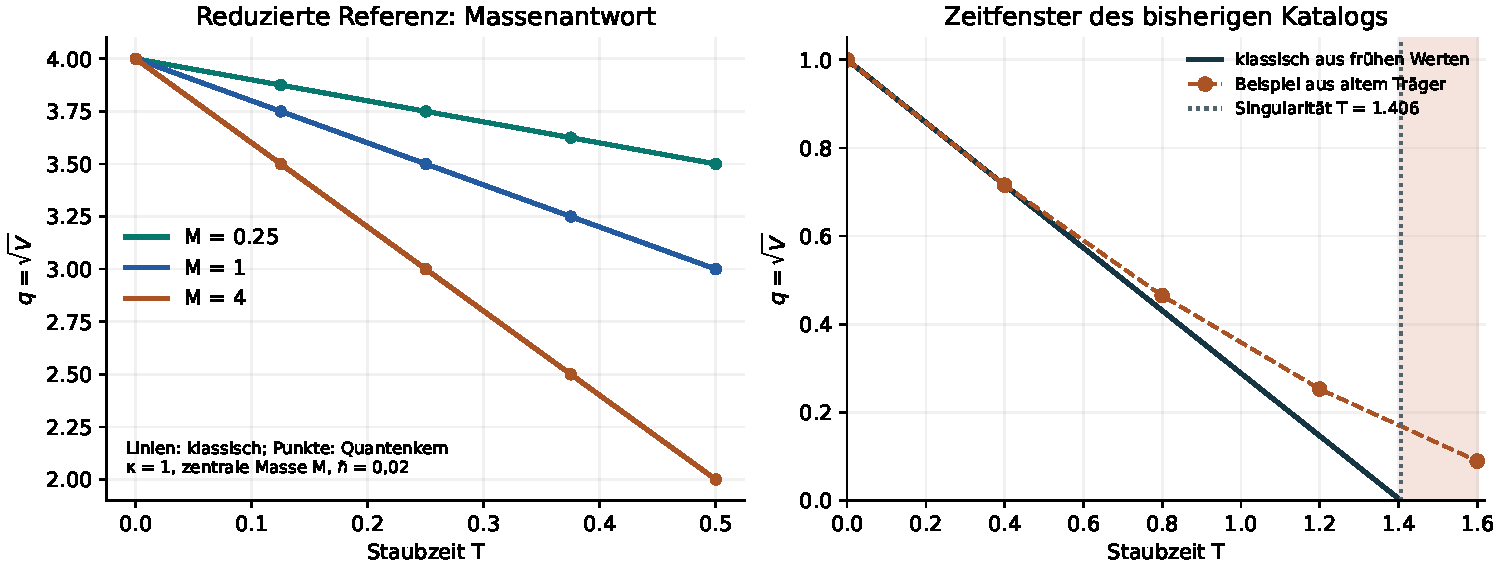
\includegraphics[width=\linewidth]{figures/classical_checks.pdf}\par
{\small\color{muted}Links: klassische Massenantwort und Schwerpunkt der propagierten Packung. Rechts: der zulässige klassische Vergleich endet vor dem letzten Zeitpunkt des alten positiven Historienkatalogs. Die gestrichelte Beispielkurve ist keine dynamische Vorhersage.\par}

\begin{tabularx}{\linewidth}{@{}p{59mm}Y@{}}\toprule
\textbf{Prüfung} & \textbf{Gemessener Befund}\\\midrule
Diskrete stationäre Wirkung & Drei Massen auf nichtäquidistantem Zeitgitter; erste Variation mit rationaler Arithmetik exakt null, lokale quadratische Änderung exakt bestätigt.\\
Unabhängige Beschleunigungsintegration & $\ddot a=-8\kappa M/(9a^2)$ bei $V_0=1$, RK4 mit 20, 40, 80 Schritten: maximaler $q$-Fehler $1{,}57\cdot10^{-8}$; bei 80 Schritten $6{,}13\cdot10^{-11}$.\\
Spektraler Quantenkern & Dirichlet-Intervall $0<q<12$, 1024/2048 innere Punkte, fünf Zeiten: 90 Auswertungen; maximale Normabweichung $1{,}45\cdot10^{-15}$.\\
Vergleich mit exakter Halbgeradenlösung & Maximaler diskreter $L^2$-Fehler $2{,}00\cdot10^{-11}$; mit 2048 Punkten $6{,}07\cdot10^{-14}$.\\
Volumen- und Masseerwartung & Maximaler Fehler gegenüber Packungsformel $2{,}26\cdot10^{-14}$ bzw. $1{,}78\cdot10^{-15}$.\\
Semiklassische Annäherung & Bei $T=1/2$ ist $\langle V\rangle-V_{\rm klass}=\hbar$: 0,04; 0,02; 0,01, für alle drei zentralen Massen.\\\bottomrule
\end{tabularx}

Die unterschiedliche Raumdiskretisierung prüft die numerische Darstellung desselben reduzierten Kerns. Sie ist keine Verfeinerung des vierdimensionalen CST-Ensembles. Die numerischen Werte sind Gleitkommakontrollen ohne neue Intervallzertifizierung. Die Vergleichsparameter wurden in einer lokalen Testspezifikation vor dem neuen Lauf festgehalten; dies war keine externe Präregistrierung.

\newpage
\kicker{04 · PRÜFUNG DER VORHANDENEN CST-DATEN}
\tit{Was die alten Historien wirklich zeigen}
\sect{A. Die 27 und 17 vorgegebenen Volumenpfade}
Die Eingaben aus [3] haben $a=w/5$, $T_j=2j/5$ und gemeinsame frühe Breiten $(5,4)$. Daraus folgt in der flachen Staubreferenz
\[
 v_0=\frac{(4/5)^{3/2}-1}{2/5}=-0{,}7111456180,\quad
 M\big|_{\kappa=1}=0{,}1264320225,\quad T_*=-1/v_0.
\]
Dies ist ein aus zwei exakten Ablesewerten \emph{implizierter klassischer} Massenwert, keine aus den alten Daten gemessene Staubmasse und keine normalisierte Quantenzustandspräparation. Bis $T=1{,}2$ gilt klassisch $q=(1,\,0{,}715542,\,0{,}431084,\,0{,}146625)$.

Keiner der 44 diskreten Pfade erfüllt an allen inneren Marken die reduzierte stationäre Gleichung. Der Entwicklungsverlauf $(5,4,3,2,1)$ hat vor der Singularität den kleinsten maximalen relativen Fehler seiner Segmentsteigungen: 25,55\,\%. Bei den 17 Prüfpfaden beträgt das entsprechende Minimum 62,61\,\%. Das feinere Kausalraster belässt die vorgeschriebene makroskopische Bahn; es erzeugt keine feinere Auswahl möglicher Volumenbahnen.

\textbf{Reichweite:} Pfade eines Quantenintegrals dürfen einzeln von klassischen Lösungen abweichen. Das Fehlen eines exakten stationären Vertreters ist daher kein allgemeiner Ausschlusssatz. Hier fehlen jedoch ein nachgewiesen konvergenter Pfadträger, seine vollständigen Mikrofasergewichte und eine daraus bestimmte Volumenverteilung. Die Tabellen liefern keinen ausgeführten Klassik-Grenzübergang.

\sect{B. Randfamilie C: Massenantwort erneut berechnet}
Die archivierten Amplitudenpolynome aus [4] wurden für drei Maße, drei Massen und drei Kontrollen unabhängig mit komplexen Gleitkommazahlen ausgewertet. Maximaler Abstand zu archivierten Intervallmittelpunkten: $2{,}25\cdot10^{-15}$. Die frühere Intervallzertifizierung wurde nicht wiederholt.

\begin{tabularx}{\linewidth}{@{}Y r r@{}}\toprule
\textbf{Maß} & \textbf{$d$, volle Phase} & \textbf{$d$, Grav.-Phase aus}\\\midrule
Symmetriegewicht & 0,068212 & 0,020505\\
Gleiches Orbitgewicht & 0,172149 & 0,019970\\
Klassisches Wachstum $p=1/2$ & 0,084830 & 0,041548\\\bottomrule
\end{tabularx}
Hier misst $d=1-|\langle A_M,A_{4M}\rangle|^2/(\|A_M\|^2\|A_{4M}\|^2)$ eine Änderung des normierten Endvektors. In der massenblinden Kontrolle ist $d=0$. Beim Wachstumsmaß ändert sich der Diagonalanteil $q_{23}$ mit voller Phase von 0,023338 auf 0,046966; ohne Gravitationsphase von 0,760351 auf 0,762171.

\note{Das Ausschalten des BD-Phasenfaktors ist \textbf{nicht} der physikalische Grenzfall $G\to0$: Sein Koeffizient skaliert bei festem $\ell,\hbar$ wie $1/G$. Die Kontrolle zeigt eine auch ohne diese Phase vorhandene Materieinterferenz. Sie widerlegt weder Gravitation allgemein noch beweist sie deren Rückwirkung.}

\newpage
\kicker{05 · ENTSCHEIDUNG UND PRÜFBARER ANSCHLUSS}
\tit{Die Brücke zur Kausalset-Dynamik bleibt offen}
\textbf{Die ursprüngliche Frage hat eine geteilte Antwort.} Die reduzierte Einstein-Staub-Referenz enthält klassische Staubbewegung und wechselseitige Materie-Geometrie-Dynamik. Der Quantenkern hat dafür den passenden geprüften Grenzfall. Das bestätigt einen notwendigen Referenzbaustein. Es zeigt noch nicht, dass die physikalisch gewichtete Summe vierdimensionaler Kausalsets diesen Baustein hervorbringt.

\sect{Was für einen positiven CST-Befund erforderlich ist}
\begin{tabularx}{\linewidth}{@{}p{9mm}Y@{}}\toprule
\textbf{Nr.} & \textbf{Erforderliche Prüfung}\\\midrule
1 & Gemeinsamer Materie-Geometrie-Kern mit festgelegtem Maß, Gesamtwirkung, Randzuständen und konsistenten Anfangszwängen. Der BD-Kontinuumsbezug [2] allein liefert diesen Kern nicht.\\
2 & Kalibrierte räumliche Volumina zu mehreren Staubeigenzeiten aus \emph{denselben dynamischen Historien}. Endbreite und Wegeetikett der Familie C reichen dafür nicht.\\
3 & Vergleich bei mindestens zwei physikalisch übereinstimmenden Verfeinerungen auf einem festen Fenster $q_{\rm klass}\ge q_{\min}>0$. Für die bisherigen frühen Werte liegt zum Beispiel $0\le T\le0{,}8$ vor der Singularität.\\
4 & Vorhersage von Massenerhaltung, $H_a^2=8\pi G\rho/3$ und $\ddot a/a=-4\pi G\rho/3$ mit gemeinsamem Fehlerbudget. Referenzfehler, Ablesefehler, Trägerfehler und Dynamikfehler getrennt ausweisen.\\
5 & Massenvariation bei gleichem Anfangsvolumen und jeweils erfülltem Anfangszwang: $|\dot q|\propto\sqrt M$. Eine nachträglich veränderte Materiephase bei festgehaltenem Gravitationsimpuls erfüllt diesen Vergleich nicht.\\\bottomrule
\end{tabularx}

Die vorige G4-Prüfung wird deshalb aufgeteilt: \texttt{G4-REF = PASS} für die hier bedingte Referenz, \texttt{G4-CST = HOLD} für deren Herleitung aus der Summe. Ein endliches Massenantwortsignal bleibt ein diagnostischer Befund. Ein neues Bounce-Gate wird nicht gestartet.

\sect{Reproduzierbarkeit}
Das Prüfpaket enthält unveränderte verwendete Eingaben samt SHA-256-Herkunft, lokale Testspezifikation, \texttt{verify.py}, numerische Einzelwerte, \texttt{plot.py}, Abbildung und Bericht. Benötigt: Python, NumPy, SciPy; Matplotlib nur für die Abbildung, LaTeX nur für den Bericht. Der Prüflauf dauert in dieser Umgebung weniger als eine Sekunde. Es wurden keine neuen Kausalsets, Sprinkling-Ensembles oder kostenpflichtigen Rechenläufe erzeugt.

\sect{Quellen und geprüfter Projektstand}
{\small
[1] J. D. Brown, K. V. Kuchař: \emph{Dust as a Standard of Space and Time in Canonical Quantum Gravity}. Phys. Rev. D 51, 5600 (1995). \url{https://arxiv.org/abs/gr-qc/9409001}. Motivation der gekoppelten Staubreferenz; die homogene Rechnung steht hier explizit.

[2] D. M. T. Benincasa, F. Dowker: \emph{The Scalar Curvature of a Causal Set}. Phys. Rev. Lett. 104, 181301 (2010), korrigierte Fassung v4. \url{https://arxiv.org/abs/1001.2725}. Diskrete Krümmungswirkung, kein hier vorausgesetzter Beweis des gekoppelten Staubgrenzfalls.

[3] Projekt: \emph{CST Staubball Historiengewichtung v0.1}, \href{https://github.com/thomasmgfeller/x6-spectral-astrolabium/pull/235}{GitHub PR 235}.

[4] Projekt: \emph{Staubball C: Zwei Massen}, \href{https://github.com/thomasmgfeller/x6-spectral-astrolabium/pull/214}{GitHub PR 214}. Archiv und Tabellen vom unveränderten Main-Stand \texttt{1ec2955a55565b0a29daa97053a3d3f6118d2d49}, geprüft am 5. November 2026.
}
\end{document}
